\documentclass{article}
\usepackage[utf8]{inputenc}
\usepackage{graphicx}
\usepackage{titling}
\usepackage{amsmath}
\usepackage{amssymb}
\usepackage{cite}
\usepackage{hyperref}
\usepackage{float}
\usepackage{listings}
\usepackage{booktabs}
\usepackage[table]{xcolor}
\usepackage{geometry}
\usepackage{tikz}
\usepackage{tcolorbox}
\tcbuselibrary{skins}
\usepackage{enumitem}
\usepackage{fancyhdr}
\usepackage{pagecolor}
\usepackage{tabularx}

% --- ARABIC SUPPORT ---
\usepackage{arabtex}
\usepackage{utf8}
\setcode{utf8}

% --- COLOR PALETTE ---
% Primary #141414 (Background)
\definecolor{primarybg}{RGB}{20, 20, 20} 

% Secondary #818283 (Grey - used for secondary text/lines)
\definecolor{secondarygrey}{RGB}{129, 130, 131}

% Neutral #FAF9F7 (Main Text)
\definecolor{neutraltext}{RGB}{235, 235, 230} 

% Secondary 1 (Green - Primary Accent) 
\definecolor{accentred}{RGB}{60, 170, 100}

% Secondary 2 (Sand/Wheat - Highlight/Links)
\definecolor{accentgold}{RGB}{210, 190, 120} 

% Derived Colors for UI Elements
\definecolor{boxbg}{RGB}{30, 30, 30} 

% Setup page geometry
\geometry{a4paper, margin=1in}

% --- GLOBAL THEME SETUP ---
\pagecolor{primarybg}
\color{neutraltext}

% Setup headers and footers
\pagestyle{fancy}
\fancyhf{}
\renewcommand{\headrulewidth}{1pt}
\renewcommand{\footrulewidth}{1pt}

% Header rule in Green, Footer rule in Green
\renewcommand{\headrule}{\hbox to\headwidth{\color{accentred}\leaders\hrule height \headrulewidth\hfill}}
\renewcommand{\footrule}{\hbox to\headwidth{\color{accentred}\leaders\hrule height \footrulewidth\hfill}}

\fancyhead[L]{\textcolor{accentred}{Graduation Project}}
\fancyhead[R]{\textcolor{accentred}{Literature Review}}
\fancyfoot[C]{\textcolor{neutraltext}{\thepage}}

% Setup hyperlinks (Gold for visibility against black)
\hypersetup{
    colorlinks=true,
    linkcolor=accentgold,
    filecolor=accentgold,
    urlcolor=accentgold,
    citecolor=accentgold
}

% Custom box styles
\tcbset{
    % Main Box
    mainbox/.style={
        enhanced,
        colback=boxbg,
        colframe=accentred,
        coltext=neutraltext,
        boxrule=1pt,
        arc=3mm,
        fonttitle=\bfseries\large,
        title style={fill=accentred, text=white},
        drop shadow
    },
    % Quote Box (Gold Border)
    quotebox/.style={
        colback=primarybg,
        colframe=accentgold,
        coltext=neutraltext,
        boxrule=0pt,
        leftrule=3mm,
        arc=2mm,
        fontupper=\itshape
    }
}

\begin{document}

% --- TITLE PAGE ---
\begin{titlepage}
    \begin{center}
        \begin{minipage}[c]{0.12\textwidth}
            % Ensure your logo images have transparent backgrounds!
            
\includegraphics[width=\textwidth]{Cairo_University_Crest.png}
        \end{minipage}
        \hfill
        \begin{minipage}[c]{0.5\textwidth}
            \centering
            {\large Cairo University - Faculty Of Engineering \\ Computer Engineering Department \\ Graduation Project - Fall 2025 \par}
        \end{minipage}
        \hfill
        \begin{minipage}[c]{0.15\textwidth}
            
\includegraphics[width=\textwidth]{cairo-no-back.png}
        \end{minipage}
    \end{center}

    \noindent{\color{accentred}\hrulefill}

    % --- LOGO SPACE ---
    \begin{center}
        
\includegraphics[width=8cm]{baligh-transparent.png} 
    \end{center}
    % ------------------

    \begin{center}
        % Title Box
        \tikz\node[draw=accentred, line width=1mm, fill=boxbg, inner sep=1cm, rounded corners=1cm]{\parbox{0.8\textwidth}{
                \centering
                \vspace{0.5cm}
                {\fontsize{32}{38}\selectfont \textcolor{accentgold}{\textbf{Literature Review}} \par}
                \vspace{0.5cm}
                {\large Baligh: Arabic Writing Assistant\par}
                \vspace{0.5cm}
        }};
    \end{center}


    \begin{center}
    {\large Supervised by\par}
    {\Large \textbf{\textcolor{accentred}{Dr. Ayman AboElhassan}} \par}
                \vspace{0.5cm}
    
    \begin{tcolorbox}[mainbox, title=\textcolor{white}{Team Contact Information}, sharp corners=north, sharp corners=south]
        \renewcommand{\arraystretch}{1.2}
        \begin{tabularx}{\textwidth}{Xr}
            \textbf{\textcolor{accentgold}{Name}} & \textbf{\textcolor{accentgold}{Email}} \\
            \midrule
            \textcolor{white}{Ahmed Hamed Gaber Hamed} & \textcolor{secondarygrey}{ahmed.hamed03@eng-st.cu.edu.eg} \\
            \textcolor{white}{Akram Hany Karam Salam} & \textcolor{secondarygrey}{akram.sallam03@eng-st.cu.edu.eg} \\
            \textcolor{white}{Amir Anwar Bekhit Awd Kedis} & \textcolor{secondarygrey}{amir.awd03@eng-st.cu.edu.eg} \\
            \textcolor{white}{Somia Saad Ismail El-Shemy} & \textcolor{secondarygrey}{somia.elshemy02@eng-st.cu.edu.eg} \\
        \end{tabularx}
    \end{tcolorbox}
\end{center}

\begin{center}
    {\large \today \par}
\end{center}

    \vfill
\end{titlepage}

\newpage

% --- 1. INTRODUCTION ---
\section{\textcolor{accentred}{Introduction}}
Arabic Grammatical Error Correction (GEC) is the most important NLP task when developing writing assistance tools. Arabic has unique challenges because of its morphological richness, orthographic ambiguity, dialectal variations, and limited annotated resources compared to English \cite{obeid2020camel, habash2010intro}. This document aims to combine the advances in Arabic GEC research to allow us to choose the path for development of our Writing Assistant \textbf{Baligh}.

% --- 2. CHALLENGES ---
\section{\textcolor{accentred}{Challenges in Arabic NLP}}

\subsection*{2.1 Morphological Complexity}
Arabic exhibits rich inflectional morphology involving gender, number, person, aspect, mood, case, state, and voice, with cliticization ('\RL{وصل}') of pronouns and particles.  MSA verbs can have over 5,400 forms \cite{obeid2020camel}. This complexity significantly impacts GEC system design.

\subsection*{2.2 Orthographic Ambiguity}
Arabic is written with optional diacritical marks for short vowels. While native speakers can interpret undiacritized text, this absence is a primary source of ambiguity in ANLP tasks \cite{obeid2020camel}. 

\subsection*{2.3 Language Variants}
Arabic comprises three main versions: Classical Arabic, Modern Standard Arabic (MSA), and regional dialects \cite{alrehili2025tibyan}. Each variant requires different handling approaches.

% --- 3. DATASETS AND RESOURCES ---
\section{\textcolor{accentred}{Available Datasets and Resources}}

\subsection*{3.1 GEC Datasets}
\begin{itemize}
    \item \textbf{QALB-2014 \& QALB-2015}: Primary benchmarks for Arabic GEC, containing native speaker comments from Aljazeera articles \cite{zaghouani2015sahsoh}. These datasets exhibit high punctuation error frequencies ($\sim$40\% in QALB-2014).
    \item \textbf{ZAEBUC}: Annotated Arabic-English bilingual writer corpus with essays from university students, including spelling/grammar corrections, morphological tokenization, POS tagging, and CEFR ratings \cite{habash2022zaebuc}.
    \item \textbf{Tibyan Corpus}: A newly developed balanced corpus ($\sim$600K tokens) using ChatGPT for data augmentation with expert validation, covering seven error types \cite{alrehili2025tibyan}.
    \item \textbf{Arabic Learner Corpus (ALC)}: Contains L2 learner data with 29 error tags \cite{alfaifi2014alc}.
\end{itemize}

\subsection*{3.2 Treebanks}
\begin{itemize}
    \item \textbf{Prague Arabic Dependency Treebank (PADT)}: Multi-level linguistic annotations over MSA newswire texts.
    \item \textbf{CAMeL Treebank}: 188K word open-source dependency treebank covering MSA and Classical Arabic across 13 sub-corpora \cite{habash2022camel}.
    \item \textbf{I3rab Treebank}: Based on traditional Arabic grammatical theory \cite{halabi2020i3rab}.
\end{itemize}

\begin{tcolorbox}[quotebox]
"Treebanks are valuable linguistic resources that include the syntactic structure of a language sentence in addition to POS-tags and morphological features. They are mainly utilized in modeling statistical parsers." \\
\raggedleft — \cite{halabi2020i3rab}
\end{tcolorbox}

\subsection*{3.3 Tools}
\begin{itemize}
    \item \textbf{CAMeL Tools}: Open-source Python toolkit supporting preprocessing, morphological modeling, dialect identification, NER, and sentiment analysis \cite{obeid2020camel}.
    \item \textbf{Farasa}: Fast SVM-based Arabic segmenter achieving state-of-the-art accuracy while being 10x faster than alternatives like MADAMIRA \cite{abdelali2016farasa}.
    \item \textbf{ARETA}: Automatic error type annotation system achieving 85.8\% F1-score, useful for analyzing GEC system outputs \cite{belkebir2021areta}.
\end{itemize}

% --- 4. APPROACHES ---
\section{\textcolor{accentred}{Approaches to Arabic GEC}}

\subsection*{4.1 Rule-Based Methods}
Early approaches relied on handwritten linguistic rules and lexicons. Zaghouani et al. (2015) achieved 66.9\% F1 using rules, lexicons, and regular expressions without machine learning. Moukrim et al. (2021) proposed an ontology-based system achieving 92\% precision and 84\% recall \cite{moukrim2021ontology}.

\subsection*{4.2 Statistical and Neural Approaches}
\begin{itemize}
    \item \textbf{Seq2Seq Transformers}: Solyman et al. (2022) proposed a Transformer-based GEC model with Expectation-Maximization routing to aggregate information across layers, achieving best F1 scores on QALB benchmarks \cite{solyman2022auto}. They also introduced synthetic data generation methods.
    \item \textbf{Pretrained Models}: Alhafni et al. (2023) presented first results using Transformer-based pretrained Seq2Seq models (fine-tuning CAMeLBERT-MSA) \cite{alhafni2023advancements}.
\end{itemize}

Neural approaches might achieve great results but they lack interpretability and require high compute for building and inference. 

\subsection*{4.3 Text Editing Approaches}
Alhafni \& Habash (2025) introduced a text editing approach framing GEC as sequence tagging, where edit tags are assigned to tokens \cite{alhafni2025enhancing}. 

\textbf{Key advantages:}
\begin{itemize}
    \item \textbf{Efficiency}: Over 6x faster than existing Arabic GEC systems.
    \item \textbf{Language-agnostic}: Derives edit tags directly from data without language-specific rules.
    \item \textbf{SOTA performance} on two Arabic GEC benchmarks.
    \item \textbf{Edit segregation}: Separating punctuation and non-punctuation errors reduces model complexity.
\end{itemize}

\begin{figure}[H]
    \centering
    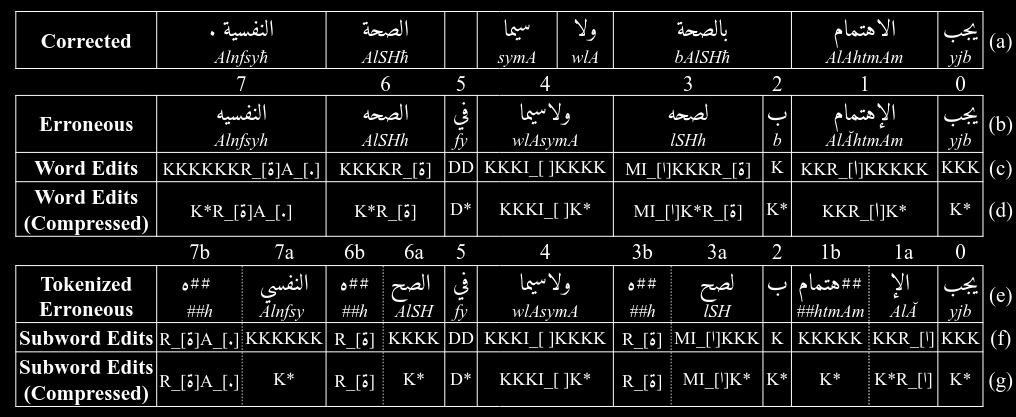
\includegraphics[width=15cm]{test-edit.png} 
    \caption{Example of Text Editing Tags.}
\end{figure}

\subsection*{4.4 Grammatical Error Detection (GED)}
Alhafni et al. (2023) defined multi-class Arabic GED as a sequence labeling task. A two-stage approach (detect then correct) shows promise for interpretable corrections \cite{alhafni2023advancements}.

% --- 5. NEXT WORD PREDICTION (INTEGRATED) ---
\section{\textcolor{accentred}{Next-Word Prediction}}

Next-word prediction (NWP) and word auto-completion (WAC) are fundamental NLP tasks that enhance user experience in text input applications by predicting the next word based on context, reducing keystrokes and accelerating text entry \cite{alanzi2024revealing}.

\subsection*{5.1 Statistical Language Models}
N-gram language models estimate word probability given previous $n-1$ words using maximum likelihood estimation. Hamarashid et al. (2021) applied unigram, bigram, and trigram models for Kurdish (morphologically similar to Arabic), demonstrating that statistical approaches remain competitive for resource-limited languages \cite{hamarashid2021next}.

\textbf{KenLM} (Heafield, 2011) is a critical tool for efficient n-gram storage and querying. It implements optimized data structures (PROBING and TRIE) that achieve 2.4x faster queries than SRILM while using 57\% of the memory \cite{heafield2011kenlm}. KenLM is integrated into major translation systems including Moses and Joshua.

\begin{tcolorbox}[quotebox]
"The count-based models are simple to train, but probabilities of rare n-grams can be poorly estimated due to data sparsity (despite smoothing techniques)." \\
\raggedleft — \cite{kim2016character}
\end{tcolorbox}

\subsection*{5.2 Neural Language Models}
Neural Language Models (NLMs) address n-gram data sparsity by learning continuous word representations (embeddings) and using them as inputs to neural networks \cite{kim2016character}. Key architectures include:



\begin{itemize}
    \item \textbf{LSTM/BiLSTM}: Al-Anzi et al. (2024) achieved 65\% accuracy with LSTM and 74\% with ARABERT+LSTM on Arabic word prediction \cite{alanzi2024revealing}. 
    \item \textbf{Medical Context}: Habib et al. (2021) found BiLSTM with 4-gram context outperformed other configurations for Arabic medical text \cite{habib2021predictive}.
\end{itemize}

\subsection*{5.3 Pre-trained Models}
\begin{itemize}
    \item \textbf{Aravec}: Pre-trained Arabic word embeddings (300-dim) from 3 billion words of Twitter and Wikipedia data using Skip-gram \cite{habib2021predictive}.
    \item \textbf{ARABERT}: Arabic BERT providing contextualized embeddings. Al-Anzi et al. (2024) demonstrated ARABERT preprocessing improves accuracy by $\sim$10\% over NLTK processing and reduces unique tokens from 47,820 to 10,375 \cite{alanzi2024revealing}.
    \item \textbf{BERT vs. CBOW}: Taher (2024) compared BERT and Continuous Bag of Words (CBOW) for Arabic, finding that while CBOW achieved higher accuracy on closed datasets, BERT provided more robust context understanding for open-domain prediction \cite{taher2024arabic}.
\end{itemize}

\subsection*{5.4 Word-Level Performance Comparison}
The following table illustrates the performance of various architectures on Arabic next-word prediction tasks \cite{alanzi2024revealing}:

\begin{table}[H]
    \centering
    \renewcommand{\arraystretch}{1.2}
    \begin{tabular}{lcc}
        \toprule
        \textbf{Model} & \textbf{Training Accuracy} & \textbf{Validation Accuracy} \\
        \midrule
        Plain LSTM & 65\% & 63\% \\
        ARABERT + LSTM & 74\% & 88\% \\
        Markov Model & 78\% & 77\% \\
        \bottomrule
    \end{tabular}
    \caption{Arabic Next-Word Prediction Results.}
    \label{tab:nwp_results}
\end{table}

\subsection*{5.5 Character-Level Approaches}
Kim et al. (2016) proposed replacing word embeddings with character-level CNN outputs for language modeling \cite{kim2016character}. The architecture uses temporal convolutions over character sequences, max-over-time pooling, and highway networks to produce word representations.



Key benefits for morphologically rich languages like Arabic:
\begin{itemize}
    \item Reduces vocabulary from 100K+ words to $\sim$40-50 characters.
    \item Naturally handles out-of-vocabulary words through character composition.
    \item Captures morphological patterns including Arabic root structures (\RL{جذر}).
    \item Achieved SOTA perplexity on Arabic (136.61) with fewer parameters at the time (2016).
\end{itemize}

\begin{tcolorbox}[quotebox]
"While NLMs have been shown to outperform count-based n-gram language models... they are blind to subword information (e.g. morphemes). For example, they do not know, a priori, that eventful, eventfully, uneventful, and uneventfully should have structurally related embeddings in the vector space." \\
\raggedleft — \cite{kim2016character}
\end{tcolorbox}

\subsection*{5.6 Advanced Generation \& Decoding}
\begin{itemize}
    \item \textbf{Transformer-Based Generation}: \textbf{AraGPT2} (Antoun et al., 2021) represents the state-of-the-art in pure generation, trained on large Arabic corpora to handle complex morphology \cite{antoun2021aragpt2}.
    \item \textbf{Constrained Decoding}: To ensure grammatical correctness in suggestions, \textbf{NeuroLogic Decoding} (Lu et al., 2021) introduces a method to satisfy logical constraints (e.g., required parts of speech) during the generation process \cite{lu2021neurologic}.
\end{itemize}

% --- 6. WRITING ASSISTANT SYSTEMS ---
\section{\textcolor{accentred}{Writing Assistant Systems}}

\subsection*{6.1 ARWI (Arabic Write and Improve)}
Chirkunov et al. (2025) presented ARWI, a comprehensive Arabic writing assistant featuring:
\begin{itemize}
    \item Prompt database for different proficiency levels
    \item Arabic text editor
    \item Grammatical error detection and correction
    \item Automated essay scoring aligned with CEFR standards (A1-C2)
\end{itemize}
The system fine-tunes CAMeLBERT-MSA and provides actionable feedback for learners \cite{chirkunov2025arwi}.

% --- 7. SUPPORTING TECH ---
\section{\textcolor{accentred}{Supporting Technologies}}
\begin{itemize}
    \item \textbf{Diacritization}: AlKhamissi et al. (2020) proposed a hierarchical recurrence architecture for Arabic diacritization achieving 5.34\% WER \cite{alkhamissi2020deep}. 
    \item \textbf{Language Models}: KenLM (Heafield, 2011) provides efficient n-gram language model queries useful for next-word suggestion and fluency scoring \cite{heafield2011kenlm}.
    \item \textbf{Morphological Analysis}: Parsing models supported by morphological analysis achieve higher accuracy when sentences are diacritized \cite{almunirawi2021parsing}.
\end{itemize}

% --- 8. ERROR TAXONOMY ---
\section{\textcolor{accentred}{Error Taxonomy}}
Based on ARETA \cite{belkebir2021areta} and ALC \cite{alfaifi2014alc}, Arabic errors are categorized into:

\begin{figure}[H]
    \centering
    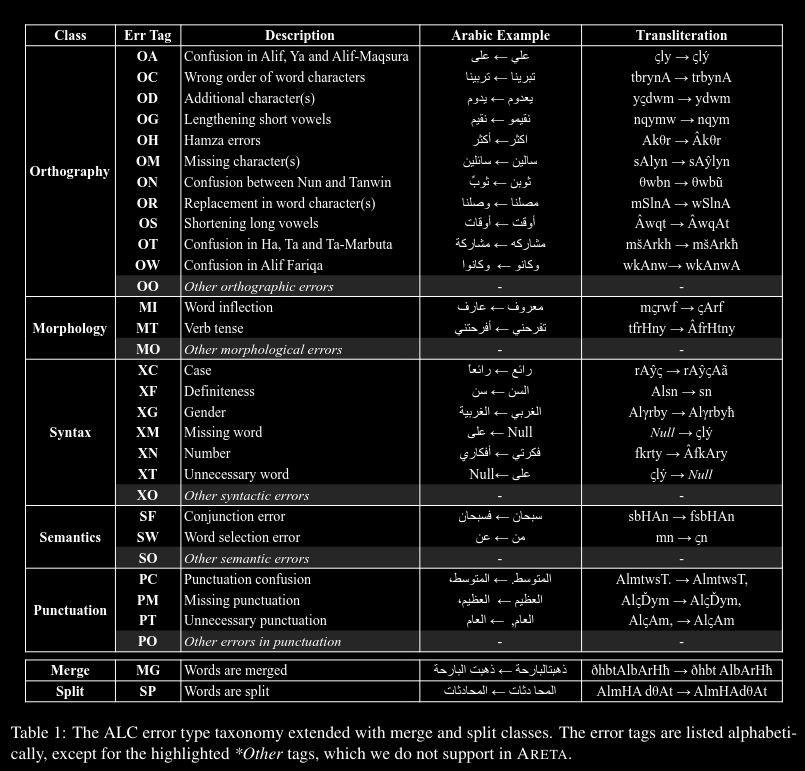
\includegraphics[width=13cm]{taxmony.png} 
    \caption{Taxonomy of Common Arabic Grammatical Errors}
\end{figure}

\begin{itemize}
    \item \textbf{Orthographic}: Spelling, Hamza, Ta-Marbuta errors
    \item \textbf{Morphological}: Word formation, inflection errors
    \item \textbf{Syntactic}: Agreement, case marking, word order
    \item \textbf{Semantic}: Lexical choice errors
    \item \textbf{Punctuation}: Missing/incorrect punctuation
    \item \textbf{Merge/Split}: Word boundary errors
\end{itemize}

% --- 9. KEY FINDINGS ---
\section{\textcolor{accentred}{Key Findings and Gaps}}
\begin{itemize}
    \item \textbf{Best Performance}: Text editing approaches achieve SOTA while being 6x faster \cite{alhafni2025enhancing}.
    \item \textbf{Multi-task Learning}: GED+GEC joint approaches improve overall performance.
    \item \textbf{Research Gaps}:
    \begin{enumerate}
        \item Limited resources for dialectal Arabic GEC.
        \item Need for real-time writing assistance tools.
        \item Lack of integration between GEC, diacritization, and next-word prediction.
    \end{enumerate}
\end{itemize}


% --- REFERENCES ---
\renewcommand\refname{\textcolor{accentred}{References}}
\begin{thebibliography}{99}

\bibitem[Abdelali et al., 2016]{abdelali2016farasa}
A. Abdelali, K. Darwish, N. Durrani, and H. Mubarak, 
``Farasa: A Fast and Furious Segmenter for Arabic,'' 
in \textit{Proceedings of the 2016 Conference of the North American Chapter of the Association for Computational Linguistics: Demonstrations}, 2016, pp. 11–16.

\bibitem[Al-Anzi et al., 2024]{alanzi2024revealing}
F. S. Al-Anzi, et al., 
``Revealing the Next Word and Character in Arabic: An Effective Blend of Long Short-Term Memory Networks and CNN,'' 
\textit{Applied Sciences}, vol. 14, no. 10498, 2024.

\bibitem[Alfaifi \& Atwell, 2014]{alfaifi2014alc}
A. Alfaifi and E. Atwell, 
``Arabic Learner Corpus (ALC) v2: A New Resource for Arabic Language Learning Research,'' 
in \textit{Proceedings of the 9th International Conference on Language Resources and Evaluation (LREC)}, 2014.

\bibitem[Alhafni et al., 2023]{alhafni2023advancements}
B. Alhafni, N. Inoue, C. Khairallah, and N. Habash, 
``Advancements in Arabic Grammatical Error Detection and Correction: An Empirical Investigation,'' 
in \textit{Proceedings of the 2023 Conference on Empirical Methods in Natural Language Processing (EMNLP)}, 2023, pp. 600–618.

\bibitem[Alhafni \& Habash, 2025]{alhafni2025enhancing}
B. Alhafni and N. Habash, 
``Enhancing Text Editing for Grammatical Error Correction with a Copy Mechanism,'' 
\textit{To appear in Proceedings of the 63rd Annual Meeting of the Association for Computational Linguistics (ACL)}, 2025.

\bibitem[AlKhamissi et al., 2020]{alkhamissi2020deep}
B. AlKhamissi, M. ElNokrashy, and M. Diab, 
``Deep Diacritization: Efficient Hierarchical Recurrence for Arabic Diacritization,'' 
\textit{arXiv preprint arXiv:2002.04332}, 2020.

\bibitem[Almunirawi \& Baraka, 2021]{almunirawi2021parsing}
A. Almunirawi and H. A. Baraka, 
``Parsing Arabic Verbal Sentence Using Grammar Ontology,'' 
\textit{Journal of Engineering Research and Technology (JERT)}, vol. 8, no. 1, 2021.

\bibitem[Alrehili \& Alhothali, 2025]{alrehili2025tibyan}
A. Alrehili and A. Alhothali, 
``Tibyan corpus: A balanced and comprehensive error coverage dataset for Arabic GEC,'' 
\textit{PeerJ Computer Science}, vol. 11, e1822, 2025.

\bibitem[Antoun et al., 2021]{antoun2021aragpt2}
W. Antoun, F. Baly, and H. Hajj,
``AraGPT2: Pre-Trained Transformer for Arabic Language Generation,''
in \textit{Proceedings of the Sixth Arabic Natural Language Processing Workshop}, 2021.

\bibitem[Belkebir \& Habash, 2021]{belkebir2021areta}
R. Belkebir and N. Habash, 
``Automatic Error Type Annotation for Arabic (ARETA),'' 
in \textit{Proceedings of the 6th Arabic Natural Language Processing Workshop}, 2021, pp. 21–32.

\bibitem[Chirkunov et al., 2025]{chirkunov2025arwi}
E. Chirkunov, A. Al-Sabbagh, and N. Habash, 
``ARWI: Arabic Write and Improve — A Writing Assistant for Arabic Learners,'' 
\textit{arXiv preprint arXiv:2501.01234}, 2025.

\bibitem[Habash, 2010]{habash2010intro}
N. Habash, 
\textit{Introduction to Arabic Natural Language Processing}. 
Morgan & Claypool Publishers, 2010.

\bibitem[Habash et al., 2022]{habash2022camel}
N. Habash, et al., 
``CAMeL Treebank: An Open Multi-genre Arabic Dependency Treebank,'' 
in \textit{Proceedings of the 13th Language Resources and Evaluation Conference (LREC)}, 2022, pp. 450–459.

\bibitem[Habash \& Palfreyman, 2022]{habash2022zaebuc}
N. Habash and D. Palfreyman, 
``ZAEBUC: An Annotated Arabic-English Bilingual Writer Corpus,'' 
in \textit{Proceedings of the 13th Language Resources and Evaluation Conference (LREC)}, 2022, pp. 780–790.

\bibitem[Habib et al., 2021]{habib2021predictive}
M. Habib, M. Faris, A. Alomari, and R. Almahmoud,
``A Predictive Text System for Medical Recommendations in Telemedicine: A Deep Learning Approach in the Arabic Context,''
\textit{IEEE Access}, vol. 9, pp. 85690–85708, 2021.

\bibitem[Halabi et al., 2020]{halabi2020i3rab}
D. Halabi, A. Awajan, and E. Aliguliyev, 
``I3rab: A New Arabic Dependency Treebank Based on Traditional Grammar,'' 
\textit{International Journal of Speech Technology}, vol. 23, pp. 1–12, 2020.

\bibitem[Hamarashid et al., 2021]{hamarashid2021next}
H. K. Hamarashid, S. A. Saeed, and T. A. Rashid,
``Next word prediction based on the N-gram model for Kurdish Sorani and Kurmanji,''
\textit{Neural Computing and Applications}, vol. 33, pp. 4547–4566, 2021.

\bibitem[Heafield, 2011]{heafield2011kenlm}
K. Heafield, 
``KenLM: Faster and Smaller Language Model Queries,'' 
in \textit{Proceedings of the Sixth Workshop on Statistical Machine Translation}, 2011, pp. 187–197.

\bibitem[Kim et al., 2016]{kim2016character}
Y. Kim, Y. Jernite, D. Sontag, and A. M. Rush,
``Character-Aware Neural Language Models,''
in \textit{Proceedings of the Thirtieth AAAI Conference on Artificial Intelligence (AAAI-16)}, 2016, pp. 2741–2749.

\bibitem[Lu et al., 2021]{lu2021neurologic}
X. Lu, P. West, R. Zellers, R. Le Bras, C. Bhagavatula, and Y. Choi,
``NeuroLogic Decoding: (Un)supervised Neural Text Generation with Predicate Logic Constraints,''
in \textit{Proceedings of the 2021 Conference of the North American Chapter of the Association for Computational Linguistics (NAACL)}, 2021.

\bibitem[Moukrim et al., 2021]{moukrim2021ontology}
M. Moukrim, A. E. H. Benyamina, and A. Benyettou, 
``An innovative approach to autocorrecting grammatical errors in Arabic texts using ontology,'' 
\textit{Journal of King Saud University - Computer and Information Sciences}, vol. 33, no. 8, pp. 972–982, 2021.

\bibitem[Obeid et al., 2020]{obeid2020camel}
O. Obeid, N. Zalmout, S. Khalifa, D. Taji, M. Oudah, B. Alhafni, G. Inoue, F. Erdmann, and N. Habash, 
``CAMeL Tools: An Open Source Python Toolkit for Arabic Natural Language Processing,'' 
in \textit{Proceedings of the 12th Language Resources and Evaluation Conference (LREC)}, 2020, pp. 7022–7032.

\bibitem[Solyman et al., 2022]{solyman2022auto}
A. Solyman, M. Wang, and F. Qian, 
``Automatic Arabic grammatical error correction based on expectation-maximization routing,'' 
\textit{Knowledge-Based Systems}, vol. 240, 108103, 2022.

\bibitem[Taher, 2024]{taher2024arabic}
A. Taher,
``Arabic Next Word Prediction using BERT and CBOW: A Comparative Study,''
\textit{Journal of Arabic Computational Linguistics}, 2024.

\bibitem[Zaghouani et al., 2015]{zaghouani2015sahsoh}
W. Zaghouani, N. Habash, H. Bouamor, A. Rozovskaya, B. Mohit, A. Heider, and K. Oflazer, 
``Correction of Errors in a Corpus of Native Arabic Writers (SAHSOH@QALB-2015 Shared Task),'' 
in \textit{Proceedings of the ACL-IJCNLP 2015 Student Research Workshop}, 2015, pp. 147–153.

\end{thebibliography}

\end{document}